% Created by tikzDevice version 0.12.3.1 on 2021-05-22 21:10:22
% !TEX encoding = UTF-8 Unicode
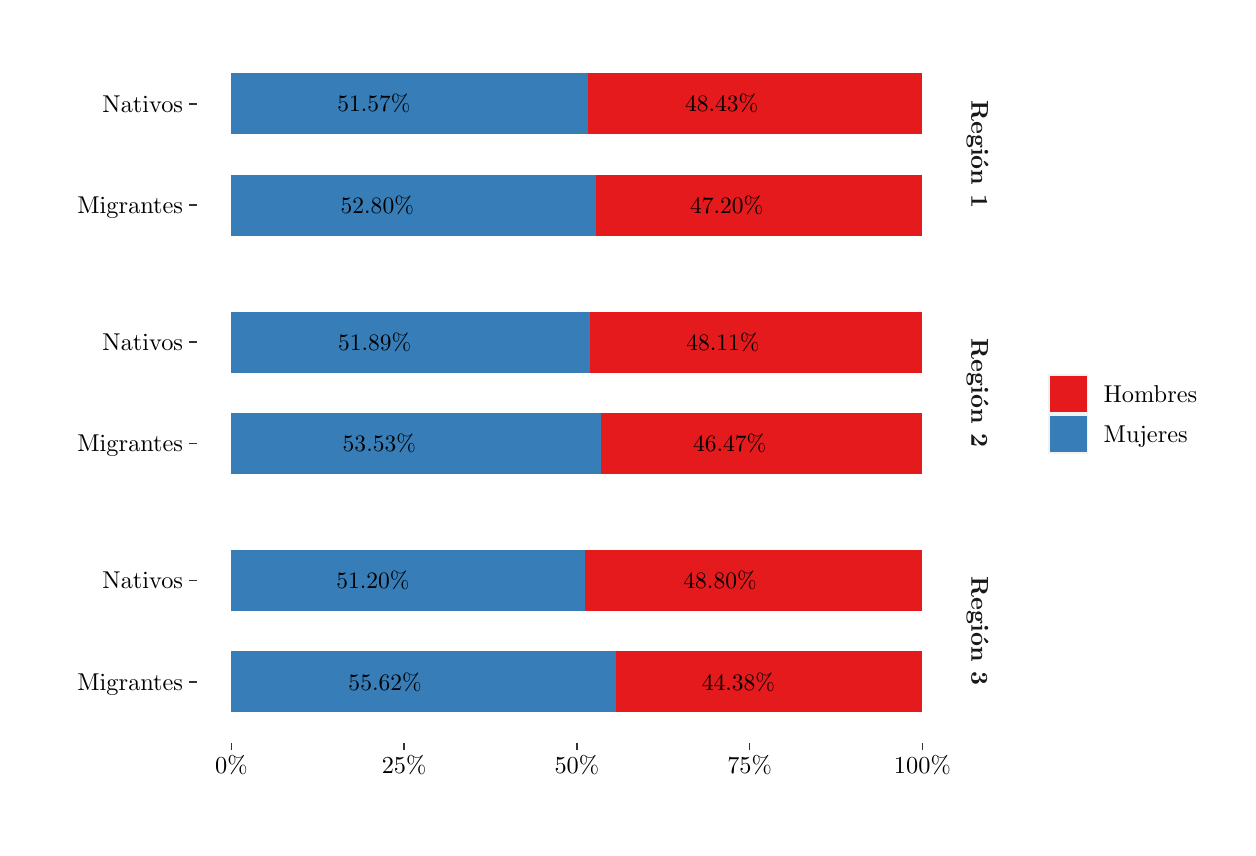
\begin{tikzpicture}[x=1pt,y=1pt]
\definecolor{fillColor}{RGB}{255,255,255}
\path[use as bounding box,fill=fillColor,fill opacity=0.00] (0,0) rectangle (433.62,289.08);
\begin{scope}
\path[clip] (  0.00,  0.00) rectangle (433.62,289.08);
\definecolor{drawColor}{RGB}{255,255,255}
\definecolor{fillColor}{RGB}{255,255,255}

\path[draw=drawColor,line width= 0.6pt,line join=round,line cap=round,fill=fillColor] (  0.00,  0.00) rectangle (433.62,289.08);
\end{scope}
\begin{scope}
\path[clip] ( 61.11,202.95) rectangle (335.80,283.58);
\definecolor{drawColor}{RGB}{255,255,255}

\path[draw=drawColor,line width= 0.3pt,line join=round] (104.81,202.95) --
	(104.81,283.58);

\path[draw=drawColor,line width= 0.3pt,line join=round] (167.24,202.95) --
	(167.24,283.58);

\path[draw=drawColor,line width= 0.3pt,line join=round] (229.67,202.95) --
	(229.67,283.58);

\path[draw=drawColor,line width= 0.3pt,line join=round] (292.10,202.95) --
	(292.10,283.58);

\path[draw=drawColor,line width= 0.6pt,line join=round] ( 61.11,224.94) --
	(335.80,224.94);

\path[draw=drawColor,line width= 0.6pt,line join=round] ( 61.11,261.59) --
	(335.80,261.59);

\path[draw=drawColor,line width= 0.6pt,line join=round] ( 73.60,202.95) --
	( 73.60,283.58);

\path[draw=drawColor,line width= 0.6pt,line join=round] (136.03,202.95) --
	(136.03,283.58);

\path[draw=drawColor,line width= 0.6pt,line join=round] (198.45,202.95) --
	(198.45,283.58);

\path[draw=drawColor,line width= 0.6pt,line join=round] (260.88,202.95) --
	(260.88,283.58);

\path[draw=drawColor,line width= 0.6pt,line join=round] (323.31,202.95) --
	(323.31,283.58);
\definecolor{fillColor}{RGB}{228,26,28}

\path[fill=fillColor] (205.44,213.94) rectangle (323.31,235.93);
\definecolor{fillColor}{RGB}{55,126,184}

\path[fill=fillColor] ( 73.60,213.94) rectangle (205.44,235.93);
\definecolor{fillColor}{RGB}{228,26,28}

\path[fill=fillColor] (202.38,250.59) rectangle (323.31,272.58);
\definecolor{fillColor}{RGB}{55,126,184}

\path[fill=fillColor] ( 73.60,250.59) rectangle (202.38,272.58);
\definecolor{drawColor}{RGB}{0,0,0}

\node[text=drawColor,anchor=base,inner sep=0pt, outer sep=0pt, scale=  0.85] at (252.59,222.00) {47.20{\%}};

\node[text=drawColor,anchor=base,inner sep=0pt, outer sep=0pt, scale=  0.85] at (126.33,222.00) {52.80{\%}};

\node[text=drawColor,anchor=base,inner sep=0pt, outer sep=0pt, scale=  0.85] at (250.75,258.65) {48.43{\%}};

\node[text=drawColor,anchor=base,inner sep=0pt, outer sep=0pt, scale=  0.85] at (125.11,258.65) {51.57{\%}};
\end{scope}
\begin{scope}
\path[clip] ( 61.11,116.82) rectangle (335.80,197.45);
\definecolor{drawColor}{RGB}{255,255,255}

\path[draw=drawColor,line width= 0.3pt,line join=round] (104.81,116.82) --
	(104.81,197.45);

\path[draw=drawColor,line width= 0.3pt,line join=round] (167.24,116.82) --
	(167.24,197.45);

\path[draw=drawColor,line width= 0.3pt,line join=round] (229.67,116.82) --
	(229.67,197.45);

\path[draw=drawColor,line width= 0.3pt,line join=round] (292.10,116.82) --
	(292.10,197.45);

\path[draw=drawColor,line width= 0.6pt,line join=round] ( 61.11,138.81) --
	(335.80,138.81);

\path[draw=drawColor,line width= 0.6pt,line join=round] ( 61.11,175.46) --
	(335.80,175.46);

\path[draw=drawColor,line width= 0.6pt,line join=round] ( 73.60,116.82) --
	( 73.60,197.45);

\path[draw=drawColor,line width= 0.6pt,line join=round] (136.03,116.82) --
	(136.03,197.45);

\path[draw=drawColor,line width= 0.6pt,line join=round] (198.45,116.82) --
	(198.45,197.45);

\path[draw=drawColor,line width= 0.6pt,line join=round] (260.88,116.82) --
	(260.88,197.45);

\path[draw=drawColor,line width= 0.6pt,line join=round] (323.31,116.82) --
	(323.31,197.45);
\definecolor{fillColor}{RGB}{228,26,28}

\path[fill=fillColor] (207.27,127.81) rectangle (323.31,149.80);
\definecolor{fillColor}{RGB}{55,126,184}

\path[fill=fillColor] ( 73.60,127.81) rectangle (207.27,149.80);
\definecolor{fillColor}{RGB}{228,26,28}

\path[fill=fillColor] (203.16,164.46) rectangle (323.31,186.45);
\definecolor{fillColor}{RGB}{55,126,184}

\path[fill=fillColor] ( 73.60,164.46) rectangle (203.16,186.45);
\definecolor{drawColor}{RGB}{0,0,0}

\node[text=drawColor,anchor=base,inner sep=0pt, outer sep=0pt, scale=  0.85] at (253.68,135.87) {46.47{\%}};

\node[text=drawColor,anchor=base,inner sep=0pt, outer sep=0pt, scale=  0.85] at (127.07,135.87) {53.53{\%}};

\node[text=drawColor,anchor=base,inner sep=0pt, outer sep=0pt, scale=  0.85] at (251.22,172.52) {48.11{\%}};

\node[text=drawColor,anchor=base,inner sep=0pt, outer sep=0pt, scale=  0.85] at (125.42,172.52) {51.89{\%}};
\end{scope}
\begin{scope}
\path[clip] ( 61.11, 30.69) rectangle (335.80,111.32);
\definecolor{drawColor}{RGB}{255,255,255}

\path[draw=drawColor,line width= 0.3pt,line join=round] (104.81, 30.69) --
	(104.81,111.32);

\path[draw=drawColor,line width= 0.3pt,line join=round] (167.24, 30.69) --
	(167.24,111.32);

\path[draw=drawColor,line width= 0.3pt,line join=round] (229.67, 30.69) --
	(229.67,111.32);

\path[draw=drawColor,line width= 0.3pt,line join=round] (292.10, 30.69) --
	(292.10,111.32);

\path[draw=drawColor,line width= 0.6pt,line join=round] ( 61.11, 52.68) --
	(335.80, 52.68);

\path[draw=drawColor,line width= 0.6pt,line join=round] ( 61.11, 89.33) --
	(335.80, 89.33);

\path[draw=drawColor,line width= 0.6pt,line join=round] ( 73.60, 30.69) --
	( 73.60,111.32);

\path[draw=drawColor,line width= 0.6pt,line join=round] (136.03, 30.69) --
	(136.03,111.32);

\path[draw=drawColor,line width= 0.6pt,line join=round] (198.45, 30.69) --
	(198.45,111.32);

\path[draw=drawColor,line width= 0.6pt,line join=round] (260.88, 30.69) --
	(260.88,111.32);

\path[draw=drawColor,line width= 0.6pt,line join=round] (323.31, 30.69) --
	(323.31,111.32);
\definecolor{fillColor}{RGB}{228,26,28}

\path[fill=fillColor] (212.48, 41.68) rectangle (323.31, 63.67);
\definecolor{fillColor}{RGB}{55,126,184}

\path[fill=fillColor] ( 73.60, 41.68) rectangle (212.48, 63.67);
\definecolor{fillColor}{RGB}{228,26,28}

\path[fill=fillColor] (201.44, 78.33) rectangle (323.31,100.32);
\definecolor{fillColor}{RGB}{55,126,184}

\path[fill=fillColor] ( 73.60, 78.33) rectangle (201.44,100.32);
\definecolor{drawColor}{RGB}{0,0,0}

\node[text=drawColor,anchor=base,inner sep=0pt, outer sep=0pt, scale=  0.85] at (256.81, 49.74) {44.38{\%}};

\node[text=drawColor,anchor=base,inner sep=0pt, outer sep=0pt, scale=  0.85] at (129.15, 49.74) {55.62{\%}};

\node[text=drawColor,anchor=base,inner sep=0pt, outer sep=0pt, scale=  0.85] at (250.19, 86.39) {48.80{\%}};

\node[text=drawColor,anchor=base,inner sep=0pt, outer sep=0pt, scale=  0.85] at (124.74, 86.39) {51.20{\%}};
\end{scope}
\begin{scope}
\path[clip] (335.80,202.95) rectangle (352.37,283.58);
\definecolor{drawColor}{gray}{0.10}

\node[text=drawColor,rotate=-90.00,anchor=base,inner sep=0pt, outer sep=0pt, scale=  0.88] at (341.05,243.26) {\textbf{Región 1}};
\end{scope}
\begin{scope}
\path[clip] (335.80,116.82) rectangle (352.37,197.45);
\definecolor{drawColor}{gray}{0.10}

\node[text=drawColor,rotate=-90.00,anchor=base,inner sep=0pt, outer sep=0pt, scale=  0.88] at (341.05,157.13) {\textbf{Región 2}};
\end{scope}
\begin{scope}
\path[clip] (335.80, 30.69) rectangle (352.37,111.32);
\definecolor{drawColor}{gray}{0.10}

\node[text=drawColor,rotate=-90.00,anchor=base,inner sep=0pt, outer sep=0pt, scale=  0.88] at (341.05, 71.00) {\textbf{Región 3}};
\end{scope}
\begin{scope}
\path[clip] (  0.00,  0.00) rectangle (433.62,289.08);
\definecolor{drawColor}{gray}{0.20}

\path[draw=drawColor,line width= 0.6pt,line join=round] ( 73.60, 27.94) --
	( 73.60, 30.69);

\path[draw=drawColor,line width= 0.6pt,line join=round] (136.03, 27.94) --
	(136.03, 30.69);

\path[draw=drawColor,line width= 0.6pt,line join=round] (198.45, 27.94) --
	(198.45, 30.69);

\path[draw=drawColor,line width= 0.6pt,line join=round] (260.88, 27.94) --
	(260.88, 30.69);

\path[draw=drawColor,line width= 0.6pt,line join=round] (323.31, 27.94) --
	(323.31, 30.69);
\end{scope}
\begin{scope}
\path[clip] (  0.00,  0.00) rectangle (433.62,289.08);
\definecolor{drawColor}{RGB}{0,0,0}

\node[text=drawColor,anchor=base,inner sep=0pt, outer sep=0pt, scale=  0.88] at ( 73.60, 19.68) {0{\%}};

\node[text=drawColor,anchor=base,inner sep=0pt, outer sep=0pt, scale=  0.88] at (136.03, 19.68) {25{\%}};

\node[text=drawColor,anchor=base,inner sep=0pt, outer sep=0pt, scale=  0.88] at (198.45, 19.68) {50{\%}};

\node[text=drawColor,anchor=base,inner sep=0pt, outer sep=0pt, scale=  0.88] at (260.88, 19.68) {75{\%}};

\node[text=drawColor,anchor=base,inner sep=0pt, outer sep=0pt, scale=  0.88] at (323.31, 19.68) {100{\%}};
\end{scope}
\begin{scope}
\path[clip] (  0.00,  0.00) rectangle (433.62,289.08);
\definecolor{drawColor}{RGB}{0,0,0}

\node[text=drawColor,anchor=base east,inner sep=0pt, outer sep=0pt, scale=  0.88] at ( 56.16,221.91) {Migrantes};

\node[text=drawColor,anchor=base east,inner sep=0pt, outer sep=0pt, scale=  0.88] at ( 56.16,258.56) {Nativos};
\end{scope}
\begin{scope}
\path[clip] (  0.00,  0.00) rectangle (433.62,289.08);
\definecolor{drawColor}{gray}{0.20}

\path[draw=drawColor,line width= 0.6pt,line join=round] ( 58.36,224.94) --
	( 61.11,224.94);

\path[draw=drawColor,line width= 0.6pt,line join=round] ( 58.36,261.59) --
	( 61.11,261.59);
\end{scope}
\begin{scope}
\path[clip] (  0.00,  0.00) rectangle (433.62,289.08);
\definecolor{drawColor}{RGB}{0,0,0}

\node[text=drawColor,anchor=base east,inner sep=0pt, outer sep=0pt, scale=  0.88] at ( 56.16,135.78) {Migrantes};

\node[text=drawColor,anchor=base east,inner sep=0pt, outer sep=0pt, scale=  0.88] at ( 56.16,172.43) {Nativos};
\end{scope}
\begin{scope}
\path[clip] (  0.00,  0.00) rectangle (433.62,289.08);
\definecolor{drawColor}{gray}{0.20}

\path[draw=drawColor,line width= 0.6pt,line join=round] ( 58.36,138.81) --
	( 61.11,138.81);

\path[draw=drawColor,line width= 0.6pt,line join=round] ( 58.36,175.46) --
	( 61.11,175.46);
\end{scope}
\begin{scope}
\path[clip] (  0.00,  0.00) rectangle (433.62,289.08);
\definecolor{drawColor}{RGB}{0,0,0}

\node[text=drawColor,anchor=base east,inner sep=0pt, outer sep=0pt, scale=  0.88] at ( 56.16, 49.65) {Migrantes};

\node[text=drawColor,anchor=base east,inner sep=0pt, outer sep=0pt, scale=  0.88] at ( 56.16, 86.30) {Nativos};
\end{scope}
\begin{scope}
\path[clip] (  0.00,  0.00) rectangle (433.62,289.08);
\definecolor{drawColor}{gray}{0.20}

\path[draw=drawColor,line width= 0.6pt,line join=round] ( 58.36, 52.68) --
	( 61.11, 52.68);

\path[draw=drawColor,line width= 0.6pt,line join=round] ( 58.36, 89.33) --
	( 61.11, 89.33);
\end{scope}
\begin{scope}
\path[clip] (  0.00,  0.00) rectangle (433.62,289.08);
\definecolor{fillColor}{RGB}{255,255,255}

\path[fill=fillColor] (363.37,129.57) rectangle (428.12,184.69);
\end{scope}
\begin{scope}
\path[clip] (  0.00,  0.00) rectangle (433.62,289.08);
\definecolor{fillColor}{gray}{0.95}

\path[fill=fillColor] (368.87,149.53) rectangle (383.32,163.98);
\end{scope}
\begin{scope}
\path[clip] (  0.00,  0.00) rectangle (433.62,289.08);
\definecolor{fillColor}{RGB}{228,26,28}

\path[fill=fillColor] (369.58,150.24) rectangle (382.61,163.27);
\end{scope}
\begin{scope}
\path[clip] (  0.00,  0.00) rectangle (433.62,289.08);
\definecolor{fillColor}{gray}{0.95}

\path[fill=fillColor] (368.87,135.07) rectangle (383.32,149.53);
\end{scope}
\begin{scope}
\path[clip] (  0.00,  0.00) rectangle (433.62,289.08);
\definecolor{fillColor}{RGB}{55,126,184}

\path[fill=fillColor] (369.58,135.78) rectangle (382.61,148.81);
\end{scope}
\begin{scope}
\path[clip] (  0.00,  0.00) rectangle (433.62,289.08);
\definecolor{drawColor}{RGB}{0,0,0}

\node[text=drawColor,anchor=base west,inner sep=0pt, outer sep=0pt, scale=  0.88] at (388.82,153.72) {Hombres};
\end{scope}
\begin{scope}
\path[clip] (  0.00,  0.00) rectangle (433.62,289.08);
\definecolor{drawColor}{RGB}{0,0,0}

\node[text=drawColor,anchor=base west,inner sep=0pt, outer sep=0pt, scale=  0.88] at (388.82,139.27) {Mujeres};
\end{scope}
\end{tikzpicture}
